\chapter{Enterprise Deployment and Application Strategies}
\label{ch:strategies}

\section{Introduction and Background}
\label{sec:deployment_intro}

Beyond Retrieval-Augmented Generation and agentic systems, enterprises require guidance on broader deployment decisions and specialized applications. This chapter addresses RQ3: \textit{What deployment configurations, reasoning enhancement techniques, and application strategies maximize LLM effectiveness across diverse enterprise use cases?}

Building on the RAG optimization techniques established in Chapter~\ref{ch:rag} and the multi-agent reliability frameworks developed in Chapter~\ref{ch:agentic}, this chapter extends the investigation to edge deployment, reasoning enhancement, and cross-domain application patterns. The RAP metric's success in balancing quality with output characteristics motivates our development of additional domain-specific metrics, while the ASR framework's emphasis on operational reliability informs our evaluation of reasoning systems.

The research synthesizes findings from seven publications spanning edge deployment, reasoning enhancement, and cross-domain applications:

\begin{enumerate}[leftmargin=*]
    \item \textbf{LLMs at the Edge}~\cite{huang2025edge}: Performance and efficiency evaluation with Ollama on diverse hardware, evaluating models from 0.5B to 90B parameters across six hardware platforms including consumer-grade devices (IJCNN 2025)
    \item \textbf{Deploying Reasoning LLMs}~\cite{huang2025reasoning_deployment}: Cross-architecture evaluation of 17 open-weight reasoning LLMs (DeepSeek-R1, Qwen3, GPT-OSS) for sentiment analysis on consumer hardware (IEEE ICDMW 2025)
    \item \textbf{Logical Reasoning with LLMs}~\cite{huang2025logical}: Few-shot prompting and fine-tuning evaluation on Turtle Soup lateral thinking puzzles, introducing the Valid Classification Ratio metric (IEEE SSCI 2025)
    \item \textbf{Explainable Sentiment Analysis with DeepSeek-R1}~\cite{huang2025deepseek}: First comprehensive evaluation of DeepSeek-R1's explainable sentiment classification with few-shot learning (IEEE Intelligent Systems)
    \item \textbf{Task Complexity Matters}~\cite{huang2026complexity}: First large-scale study of reasoning effectiveness across 504 configurations, revealing task-complexity-dependent performance patterns and introducing Pareto frontier analysis for model selection (PAKDD 2026, Submitted)
    \item \textbf{Chinese-English Translation Optimization}~\cite{huang2025translation}: Comprehensive LLM evaluation across zero-shot, few-shot, and fine-tuned paradigms using the MAC parallel corpus (IEEE SSCI 2025)
    \item \textbf{LLM Sentiment for Soccer Betting}~\cite{samuel2025soccer}: Novel hybrid framework integrating LLM-derived sentiment features into machine learning models for sports prediction (IEEE ICDMW 2025)
\end{enumerate}

This chapter is organized around three themes: (1) edge deployment strategies for privacy-preserving and cost-effective applications, (2) reasoning enhancement techniques including few-shot prompting and fine-tuning, and (3) cross-domain applications demonstrating the generalizability of LLM optimization techniques.

\section{Edge Deployment Strategies}
\label{sec:edge_deployment}

Enterprise adoption of LLMs faces critical constraints around privacy, latency, and infrastructure costs. Edge deployment---executing models locally on consumer-grade hardware---addresses these challenges while enabling new application paradigms. The democratization of LLMs through edge deployment holds significant potential for social good: by enabling local execution, edge LLMs enhance privacy in sensitive domains like healthcare and education, reduce the environmental footprint of AI deployment, and expand access to AI in regions with limited cloud infrastructure. These considerations connect directly to the multi-agent systems explored in Chapter~\ref{ch:agentic}, where edge deployment enables privacy-preserving automation of sensitive business processes like invoice reconciliation.

\subsection{LLMs at the Edge with Ollama}
\label{subsec:ollama_edge}

\subsubsection{Motivation and Approach}

Energy efficiency is a critical consideration in deploying large language models due to their significant environmental footprint. We leverage Ollama, an open-source framework that facilitates efficient local deployment of LLMs, to evaluate performance and efficiency across diverse hardware platforms. Ollama emerges as a lightweight framework designed to simplify local LLM deployment and execution, offering an intuitive API for model management while enhancing transparency, privacy, and performance. Its cross-platform compatibility across macOS, Linux, and Windows allows organizations to leverage existing hardware for AI applications efficiently.

\subsubsection{Experimental Setup}

We evaluate open-source LLMs from the Qwen2.5 and Llama3 families (0.5B--90B parameters) across six hardware platforms spanning high-end systems, consumer laptops, and edge devices:

\begin{itemize}[leftmargin=*]
    \item \textbf{High-end Desktop GPU:} NVIDIA RTX A6000 Ada Generation (48GB GDDR6 ECC, 18,176 CUDA cores, 568 Tensor cores)
    \item \textbf{Consumer Desktop GPU:} NVIDIA GeForce RTX 4090 (24GB GDDR6X, 16,384 CUDA cores, 512 Tensor cores)
    \item \textbf{Laptop GPU:} NVIDIA GeForce RTX 4090 Laptop (16GB GDDR6, 9,728 CUDA cores, 304 Tensor cores)
    \item \textbf{Apple Silicon (High-end):} M3 Max MacBook Pro (96GB unified memory)
    \item \textbf{Apple Silicon (Mid-range):} M4 Max MacBook Pro (48GB unified memory)
    \item \textbf{Edge Device:} NVIDIA Jetson AGX Orin Developer Kit (64GB memory, 2,048 CUDA cores, 64 Tensor cores, up to 275 TOPS)
\end{itemize}

The evaluation utilizes the Global Maritime Risk Incident Dataset (GMRID) v3, chosen for its domain specificity to the maritime industry where LLM applications are relatively unexplored. This dataset builds on the maritime risk identification work described in Chapter~\ref{ch:agentic}, providing a consistent evaluation domain across multiple studies. Table~\ref{tab:ollama_models} details the evaluated models with their specifications under Ollama's Q4\_K\_M quantization.

\begin{table}[htbp]
\centering
\caption{Ollama Models Evaluated for Edge Deployment}
\label{tab:ollama_models}
\begin{tabular}{@{}lccc@{}}
\toprule
\textbf{Model} & \textbf{Size} & \textbf{Precision} & \textbf{Category} \\
\midrule
qwen2.5:0.5b & 397 MB & Q4\_K\_M & Small \\
llama3.2:1b & 1.3 GB & Q4\_K\_M & Small \\
qwen2.5:1.5b & 986 MB & Q4\_K\_M & Small \\
llama3.2:3b & 2.0 GB & Q4\_K\_M & Small \\
qwen2.5:3b & 1.9 GB & Q4\_K\_M & Small \\
qwen2.5:7b & 4.7 GB & Q4\_K\_M & Medium \\
llama3.1:8b & 4.9 GB & Q4\_K\_M & Medium \\
llama3.2-vision:11b & 7.9 GB & Q4\_K\_M & Medium \\
qwen2.5:14b & 9.0 GB & Q4\_K\_M & Medium \\
qwen2.5:32b & 19 GB & Q4\_K\_M & Medium \\
llama3.1:70b & 42 GB & Q4\_K\_M & Large \\
llama3.3:70b & 42 GB & Q4\_K\_M & Large \\
qwen2.5:72b & 47 GB & Q4\_K\_M & Large \\
llama3.2-vision:90b & 54 GB & Q4\_K\_M & Large \\
\bottomrule
\end{tabular}
\end{table}

\subsubsection{Evaluation Metrics}

We employ comprehensive metrics capturing both performance and efficiency. These metrics complement the RAP metric introduced in Chapter~\ref{ch:rag} by focusing on deployment-specific considerations rather than output quality alone:

\begin{enumerate}[leftmargin=*]
    \item \textbf{Energy per Inference:} Energy required to process a single input sequence, measured in Joules:
    \begin{equation}
    \text{Energy per Inference (J)} = \text{Time (s)} \times P_{\text{CPU+GPU}}(\text{W})
    \end{equation}
    where $P_{\text{CPU+GPU}}$ is the average power consumption during inference, excluding idle power.
    
    \item \textbf{Performance-to-Power Ratio:} Performance achieved per unit of energy consumed:
    \begin{equation}
    \text{Performance-to-Power Ratio} = \frac{\text{F1 Score (\%)}}{\text{Energy Consumed (J)}}
    \end{equation}
    
    \item \textbf{Throughput:} Tokens processed per second (t/s), enabling comparison of inference speed across platforms.
\end{enumerate}

\subsubsection{Results}

Figure~\ref{fig:energy_efficiency} presents performance and energy efficiency metrics on RTX A6000, revealing distinct trade-offs between model size, accuracy, and energy consumption.

\begin{figure*}[h!]
    \centering
    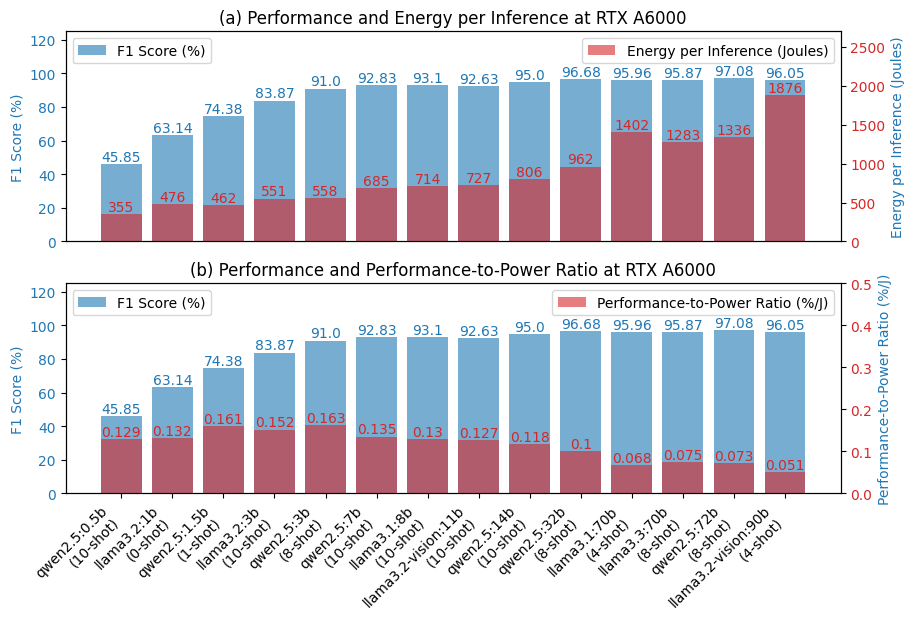
\includegraphics[width=\textwidth]{images/RTX-A6000-Perf-to-Power.png}
    \caption{Performance and Energy Efficiency Metrics on RTX A6000. (a) F1 Score (\%) vs. Energy per Inference (Joules). (b) F1 Score (\%) vs. Performance-to-Power Ratio (\%/J). Large models achieve high F1 scores but consume significantly more energy, while small models offer superior energy efficiency with acceptable performance trade-offs.}
    \label{fig:energy_efficiency}
\end{figure*}

Key findings from our comprehensive edge deployment evaluation:

\begin{enumerate}[leftmargin=*]
    \item \textbf{Quantization effectiveness:} Ollama's Q4\_K\_M quantization outperforms bitsandbytes 4-bit implementation, with llama3.1:8b achieving a mean F1 score of 92.87\% ($\pm$0.46\%) compared to its baseline of 89.50\% (3.37 percentage point improvement), and llama3.1:70b improving to 95.73\% ($\pm$0.23\%) from 95.51\% (0.22 percentage point improvement). This finding reinforces the open-source viability theme established in Chapter~\ref{ch:rag}, demonstrating that optimization techniques can unlock competitive performance from smaller models.
    
    \item \textbf{WSL performance gains:} Windows Subsystem for Linux (WSL) delivers substantial throughput improvements over native Windows. On RTX A6000, qwen2.5:0.5b processes 16,933 tokens/s on WSL compared to 816 tokens/s on Windows---a 21$\times$ speedup. This gap narrows for larger models, with differences as low as 15\% at 90B parameters.
    
    \item \textbf{Optimal model sizing:} Medium-sized models (7B--32B) achieve the best balance between performance and efficiency:
    \begin{itemize}
        \item qwen2.5:32b attains 96.75\% ($\pm$0.11\%) F1 score with practical inference speeds (mean 710 t/s across platforms)
        \item qwen2.5:7b achieves 92.64\% ($\pm$0.14\%) F1 with mean throughput of 2,873 t/s
        \item llama3.1:8b reaches 92.87\% ($\pm$0.46\%) F1 with mean throughput of 3,017 t/s
    \end{itemize}
    
    \item \textbf{Cross-platform stability:} Larger models exhibit increased cross-platform consistency, with F1 score standard deviations narrowing from 0.26--0.90\% (small models) to 0.07--0.23\% (large models), indicating more robust quantization at scale.
    
    \item \textbf{Energy trade-offs:} Large models such as qwen2.5:72b and llama3.2-vision:90b achieve high F1 scores (97.08\% and 96.05\%) but consume 1,283--1,876 Joules per inference. Small models like llama3.2-3b and qwen2.5:3b consume only 551--558 Joules while achieving 83.87\% and 91.00\% F1 respectively. Small models like qwen2.5:1.5b and qwen2.5:3b achieve the highest performance-to-power ratios (0.161 and 0.163 \%/J), ideal for energy-efficient deployments.
\end{enumerate}

Tables~\ref{tab:edge_results_small}, \ref{tab:edge_results_medium}, and \ref{tab:edge_results_large} summarize performance across hardware platforms by model category.

\begin{table}[htbp]
\centering
\caption{Edge Deployment Performance: Small Models (0.5B--3B)}
\label{tab:edge_results_small}
\resizebox{\textwidth}{!}{%
\begin{tabular}{@{}lcccc@{}}
\toprule
\textbf{Model} & \textbf{Mean F1 (\%)} & \textbf{Std (\%)} & \textbf{Mean T-put (t/s)} & \textbf{Mean Time (s)} \\
\midrule
qwen2.5:0.5b & 46.66 & 0.77 & 7,141 & 0.942 \\
llama3.2:1b & 63.17 & 0.33 & 2,033 & 1.357 \\
qwen2.5:1.5b & 74.21 & 0.90 & 3,479 & 1.038 \\
llama3.2:3b & 83.97 & 0.32 & 4,400 & 1.328 \\
qwen2.5:3b & 90.89 & 0.26 & 3,833 & 1.346 \\
\bottomrule
\end{tabular}
}
\end{table}

\begin{table}[htbp]
\centering
\caption{Edge Deployment Performance: Medium Models (7B--32B)}
\label{tab:edge_results_medium}
\resizebox{\textwidth}{!}{%
\begin{tabular}{@{}lcccc@{}}
\toprule
\textbf{Model} & \textbf{Mean F1 (\%)} & \textbf{Std (\%)} & \textbf{Mean T-put (t/s)} & \textbf{Mean Time (s)} \\
\midrule
qwen2.5:7b & 92.64 & 0.14 & 2,873 & 1.840 \\
llama3.1:8b & 92.87 & 0.46 & 3,017 & 1.785 \\
llama3.2-vision:11b & 92.89 & 0.33 & 2,950 & 1.746 \\
qwen2.5:14b & 95.00 & 0.14 & 1,629 & 3.004 \\
qwen2.5:32b & 96.75 & 0.11 & 710 & 7.781 \\
\bottomrule
\end{tabular}
}
\end{table}

\begin{table}[htbp]
\centering
\caption{Edge Deployment Performance: Large Models (70B--90B)}
\label{tab:edge_results_large}
\resizebox{\textwidth}{!}{%
\begin{tabular}{@{}lcccc@{}}
\toprule
\textbf{Model} & \textbf{Mean F1 (\%)} & \textbf{Std (\%)} & \textbf{Mean T-put (t/s)} & \textbf{Mean Time (s)} \\
\midrule
llama3.1:70b & 95.73 & 0.23 & 287 & 8.762 \\
llama3.3:70b & 95.84 & 0.07 & 368 & 16.513 \\
qwen2.5:72b & 96.90 & 0.20 & 263 & 10.660 \\
llama3.2-vision:90b & 96.04 & 0.07 & 90 & 17.739 \\
\bottomrule
\end{tabular}
}
\end{table}

\subsection{Deploying Reasoning LLMs on Consumer Hardware}
\label{subsec:reasoning_deployment}

\subsubsection{Motivation}

Deploying reasoning-enabled LLMs for sentiment analysis requires balancing accuracy, explainability, and efficiency under consumer hardware constraints. We present a cross-architecture evaluation of three reasoning model families---DeepSeek-R1, Qwen3, and GPT-OSS---spanning 17 open-weight variants. This addresses a critical gap: most existing evaluations target datacenter or cloud settings, leaving practitioners without evidence-based guidelines for consumer hardware deployment.

\subsubsection{Reasoning Intensity Metric}

We introduce Reasoning Intensity (RI) to capture trade-offs between explanation depth and computational cost:

\begin{equation}
RI = \frac{\text{Mean Reasoning Tokens (MRT)}}{\text{Mean Reasoning Tokens (MRT)} + \text{Mean Output Tokens (MOT)}}
\end{equation}

For DeepSeek-R1 models, both the \textit{reasoning content} (step-by-step thought process) and the final JSON output are included in the token count. The reasoning content refers to the complete trace of the model's thought process generated during inference, including intermediate evaluations and decision-making steps. This metric enables systematic comparison of reasoning strategies across architectures and complements the evaluation framework established in earlier chapters by capturing a dimension---reasoning overhead---not addressed by traditional accuracy metrics.

\subsubsection{Experimental Setup}

We evaluate models on fine-grained Amazon Reviews sentiment classification (5 classes: Strongly Negative, Negative, Neutral, Positive, Strongly Positive) using few-shot prompting. The primary benchmark comprises 1,838 reviews with human annotation, split 70\%/30\% for training/testing. To assess temporal robustness, we introduce Testset2: 574 manually annotated contemporary Amazon reviews collected in mid-2025.

\textbf{Model Families:}
\begin{itemize}[leftmargin=*]
    \item \textbf{DeepSeek-R1:} 8B, 14B, 32B, and 70B variants
    \item \textbf{Qwen3:} 0.6B, 1.7B, 4B, 8B, 14B, 30B, and 32B variants
    \item \textbf{GPT-OSS:} 20B and 120B, each with low/medium/high reasoning configurations
\end{itemize}

All models were executed via Ollama v0.11.4 using 4-bit quantization (MXFP4 for GPT-OSS; Q4\_K\_M for others), with a context length of 8,192 tokens.

\subsubsection{Results}

Table~\ref{tab:reasoning_deployment} presents deployment performance across model families on NVIDIA H100 GPU (96GB VRAM).

\begin{table}[htbp]
\centering
\caption{Cross-Architecture Reasoning Performance (5-Level Sentiment) on H100 GPU}
\label{tab:reasoning_deployment}
\resizebox{\textwidth}{!}{%
\begin{tabular}{@{}lccccccc@{}}
\toprule
\textbf{Model} & \textbf{F1 (\%)} & \textbf{Acc (\%)} & \textbf{MRT} & \textbf{MOT} & \textbf{RI} & \textbf{VRAM} & \textbf{Time (s)} \\
\midrule
\multicolumn{8}{c}{\textit{DeepSeek-R1 Family}} \\
\midrule
deepseek-r1:8b & 71.0 & 68.8 & 338 & 49 & 0.873 & 13 GB & 3.71 \\
deepseek-r1:14b & 77.4 & 75.5 & 248 & 54 & 0.819 & 18 GB & 4.88 \\
deepseek-r1:32b & \textbf{81.7} & \textbf{79.9} & 241 & 34 & 0.873 & 31 GB & 7.05 \\
deepseek-r1:70b & 74.2 & 71.3 & 237 & 40 & 0.855 & 58 GB & 12.08 \\
\midrule
\multicolumn{8}{c}{\textit{Qwen3 Family}} \\
\midrule
qwen3:0.6b & 65.2 & 64.8 & 236 & 72 & 0.765 & 6.1 GB & 1.34 \\
qwen3:1.7b & 75.7 & 76.8 & 217 & 57 & 0.790 & 6.8 GB & 1.56 \\
qwen3:4b & 84.3 & 83.7 & 284 & 60 & 0.825 & 11 GB & 3.93 \\
qwen3:8b & \textbf{84.8} & \textbf{84.9} & 249 & 59 & 0.807 & 13 GB & 8.35 \\
qwen3:14b & 84.6 & 83.7 & 245 & 61 & 0.799 & 19 GB & 10.20 \\
qwen3:30b & 84.3 & 84.8 & 1234 & 20 & 0.984 & 26 GB & 12.35 \\
qwen3:32b & 82.3 & 81.3 & 279 & 60 & 0.821 & 40 GB & 15.71 \\
\midrule
\multicolumn{8}{c}{\textit{GPT-OSS Family}} \\
\midrule
gpt-oss:20b (low) & 66.9 & 64.2 & 13 & 18 & 0.417 & 23 GB & 0.64 \\
gpt-oss:20b (medium) & 81.7 & 81.3 & 165 & 28 & 0.851 & 23 GB & 2.30 \\
gpt-oss:20b (high) & 84.6 & 83.8 & 744 & 30 & 0.961 & 23 GB & 8.60 \\
gpt-oss:120b (low) & 85.5 & 85.3 & 22 & 40 & 0.361 & 81 GB & 1.58 \\
gpt-oss:120b (medium) & \textbf{86.2} & \textbf{86.4} & 115 & 42 & 0.728 & 81 GB & 3.15 \\
gpt-oss:120b (high) & 83.4 & 82.8 & 679 & 43 & 0.940 & 81 GB & 11.84 \\
\bottomrule
\end{tabular}
}
\end{table}

Key findings reveal three distinct reasoning regimes:

\begin{enumerate}[leftmargin=*]
    \item \textbf{Best accuracy:} GPT-OSS achieves the highest F1 (86.2\% with gpt-oss:120b medium configuration) but requires 81 GB VRAM, far exceeding consumer GPU limits.
    
    \item \textbf{Practical balance:} Qwen3 delivers the most practical balance for consumer deployment. Within the 16GB VRAM constraint of an RTX 4090 Laptop, three models are viable:
    \begin{itemize}
        \item qwen3:8b: Optimal accuracy (84.8\% F1), 13GB VRAM, 8.35s inference
        \item qwen3:4b: Balanced performance (84.3\% F1), 11GB VRAM, 3.93s inference
        \item qwen3:1.7b: Resource-constrained option (75.7\% F1), 6.8GB VRAM, 1.56s inference
    \end{itemize}
    
    \item \textbf{Reasoning intensity patterns:} The results reveal three operational regimes:
    \begin{itemize}
        \item \textit{Minimal Reasoning} (RI $<$ 0.5): GPT-OSS low configurations prioritize throughput over explainability
        \item \textit{Balanced Reasoning} (0.5 $\leq$ RI $\leq$ 0.85): Most top-performing models operate here, including gpt-oss:120b (medium) achieving 86.2\% F1 with RI = 0.728
        \item \textit{Intensive Reasoning} (RI $>$ 0.85): DeepSeek-R1 models allocate 85--98\% of tokens to reasoning, enhancing explainability with modest accuracy gains
    \end{itemize}
    
    \item \textbf{Architecture over scale:} Larger models do not always outperform smaller counterparts. deepseek-r1:32b (81.7\% F1) substantially outperforms deepseek-r1:70b (74.2\% F1), demonstrating that architectural efficiency matters more than parameter count. This finding echoes the Orca-2-13b results from Chapter~\ref{ch:rag}, reinforcing the dissertation's broader finding that model optimization often matters more than scale.
\end{enumerate}

\subsubsection{Temporal Robustness Evaluation}

To assess model robustness under temporal drift, we evaluate on Testset2 comprising 574 manually annotated contemporary reviews from mid-2025.

\begin{table}[htbp]
\centering
\caption{Cross-Platform Temporal Robustness: Original vs. Contemporary Reviews}
\label{tab:temporal_robustness}
\resizebox{\textwidth}{!}{%
\begin{tabular}{@{}llcccc@{}}
\toprule
\textbf{Model} & \textbf{Hardware} & \textbf{Original F1 (\%)} & \textbf{Testset2 F1 (\%)} & \textbf{$\Delta$ F1} & \textbf{RI Stability} \\
\midrule
qwen3:1.7b & H100 & 75.7 & 57.9 & -17.8 & $\pm$0.012 \\
qwen3:1.7b & RTX 4090 & 72.6 & 58.1 & -14.5 & $\pm$0.010 \\
qwen3:4b & H100 & 84.3 & 67.8 & -16.5 & $\pm$0.011 \\
qwen3:4b & RTX 4090 & 81.7 & 65.7 & -16.0 & $\pm$0.001 \\
qwen3:8b & H100 & 84.8 & 72.3 & -12.5 & $\pm$0.021 \\
qwen3:8b & RTX 4090 & 82.1 & 73.3 & -8.8 & $\pm$0.017 \\
\bottomrule
\end{tabular}
}
\end{table}

Results reveal consistent 10--17 percentage point F1 degradation across models on contemporary data, though reasoning intensity remains remarkably stable ($\pm$0.02) across temporal domains. Notably, qwen3:8b exhibits superior temporal resilience, maintaining the smallest relative degradation among evaluated models. This suggests that while models' reasoning processes are robust, their learned sentiment patterns require periodic updating to account for evolving language use and product categories.

\section{Reasoning Enhancement Techniques}
\label{sec:reasoning_enhancement}

\subsection{Logical Reasoning via Lateral Thinking Puzzles}
\label{subsec:turtle_soup}

\subsubsection{The Turtle Soup Benchmark}

To assess logical reasoning capabilities, we utilize the Turtle Soup Question Answering (TSQA) dataset from the ``Logical Reasoning with LLM'' competition. The Turtle Soup game, popularized by the book \textit{Challenging Lateral Thinking Puzzles}, presents mystery puzzles requiring lateral thinking---players must deduce hidden rationales through yes/no questions. The game's name originates from a classic problem: a man orders turtle soup at a restaurant and subsequently commits suicide; players must deduce the rationale through constrained questioning.

The dataset comprises:
\begin{itemize}[leftmargin=*]
    \item 25,000 labeled training questions
    \item 3,000 labeled validation questions
    \item Chinese language content (adding complexity for primarily English-trained models)
\end{itemize}

Model responses are constrained to five categories: 是 (Yes), 不是 (No), 不重要 (Unimportant), 问法错误 (Wrong Question), and 回答正确 (Correct Answer).

\subsubsection{Methodology}

\textbf{Model Selection:} We evaluate diverse state-of-the-art LLMs including GPT-4o, o1-preview, o1-mini, Qwen2.5 (3B--72B), Llama3.1 (8B--70B), InternLM2.5 (7B, 7B-1M, 20B), and Mistral-7B. For open-source models lacking native Chinese support, we utilized their fine-tuned Chinese versions.

\textbf{Few-shot Prompting:} We employ a concise system prompt (``You are an expert in logical reasoning'') with representative examples covering all answer categories. Few-shot configurations range from 0 to 50 shots.

\textbf{Parameter-Efficient Fine-Tuning:} We apply LoRA~\cite{hu2022lora} (rank 64, alpha 128) and QLoRA~\cite{dettmers2023qlora} (4-bit quantization) for efficient adaptation on consumer-grade hardware. This approach aligns with the parameter-efficient techniques that enabled the multi-agent systems in Chapter~\ref{ch:agentic} to run on edge hardware.

\subsubsection{Valid Classification Ratio (VCR)}

We introduce the Valid Classification Ratio (VCR) as a novel metric for assessing output reliability:

\begin{equation}
VCR = \frac{\text{Number of valid classifications}}{\text{Total number of outputs}}
\end{equation}

VCR measures the proportion of responses that map to valid answer categories, capturing model reliability beyond accuracy. During evaluation, we observed that some models produce outputs containing extraneous text or failing to match predefined labels, necessitating post-processing before F1 calculation. This metric complements the Agentic Success Rate (ASR) introduced in Chapter~\ref{ch:agentic}, but focuses specifically on output validity rather than tool-calling reliability. While ASR measures whether agents successfully execute multi-step workflows, VCR measures whether models produce outputs conforming to expected formats---a prerequisite for downstream processing in production systems.

\subsubsection{Results}

Table~\ref{tab:reasoning_results} presents logical reasoning performance across few-shot and fine-tuned configurations.

\begin{table}[htbp]
\centering
\caption{Logical Reasoning Performance on TSQA Benchmark}
\label{tab:reasoning_results}
\begin{tabular}{@{}llccccc@{}}
\toprule
\textbf{Model} & \textbf{Method} & \textbf{Shots} & \textbf{Acc (\%)} & \textbf{F1 (\%)} & \textbf{VCR (\%)} \\
\midrule
GPT-4o & Few-shot & 10 & 79.12 & 80.36 & 99.2 \\
o1-preview & Few-shot & 50 & 75.89 & 77.08 & 98.7 \\
o1-mini & Few-shot & 50 & 74.56 & 75.89 & 98.4 \\
Qwen2.5-72B & Few-shot & 10 & 79.85 & \textbf{80.88} & 98.5 \\
Qwen2.5-7B & Few-shot & 50 & 74.23 & 75.45 & 97.8 \\
Qwen2.5-3B & Few-shot & 50 & 71.34 & 72.67 & 96.9 \\
Llama3.1-70B & Few-shot & 20 & 76.89 & 78.12 & 98.1 \\
Llama3.1-8B & Few-shot & 50 & 73.45 & 74.78 & 97.5 \\
InternLM2.5-7B-1M & Few-shot & 50 & 75.67 & 77.01 & 97.9 \\
InternLM2.5-7B & Few-shot & 50 & 74.12 & 75.34 & 97.6 \\
Mistral-7B & Few-shot & 50 & 72.89 & 74.12 & 97.2 \\
\midrule
Llama3.1-70B & Fine-tuned & -- & 79.65 & \textbf{80.77} & 99.1 \\
Qwen2-72B & Fine-tuned & -- & 79.21 & 80.33 & 99.0 \\
InternLM2.5-7B-1M & Fine-tuned & -- & 78.92 & 80.28 & 98.8 \\
InternLM2.5-20B & Fine-tuned & -- & 78.89 & 80.28 & 98.9 \\
InternLM2.5-7B & Fine-tuned & -- & 78.45 & 79.89 & 98.7 \\
Qwen2.5-7B & Fine-tuned & -- & 77.89 & 79.23 & 98.6 \\
\bottomrule
\end{tabular}
\end{table}

Key findings:

\begin{enumerate}[leftmargin=*]
    \item \textbf{Open-source competitiveness:} Qwen2.5-72B achieved the highest few-shot F1 score (80.88\%), surpassing GPT-4o's 80.36\% with only 10-shot prompting, demonstrating that open-source models can match or exceed proprietary alternatives on complex reasoning tasks. This reinforces the open-source viability findings from Chapter~\ref{ch:rag} where Orca-2-13b achieved comparable performance to GPT-4 in RAG applications.
    
    \item \textbf{Unexpected o1-preview performance:} The o1-preview model, despite its purported superior reasoning capabilities, exhibited lower F1 scores (77.08\%) compared to GPT-4o even with 50-shot prompting. This warrants further investigation into whether o1-preview's reasoning strengths are better suited to other task types.
    
    \item \textbf{Fine-tuning superiority:} Fine-tuning generally yields superior results, with Llama3.1-70B achieving 80.77\% F1 after fine-tuning---surpassing all few-shot configurations except Qwen2.5-72B.
    
    \item \textbf{Extended context benefit:} InternLM2.5-7B-1M, with its 1-million-token context window, demonstrated significant improvement from few-shot (77.01\%) to fine-tuned (80.28\%), ranking third overall among fine-tuned models despite its smaller parameter count.
    
    \item \textbf{VCR improvements:} Fine-tuning substantially improves VCR, with all fine-tuned models exceeding 98.6\% valid classification rates compared to 96.9--99.2\% for few-shot configurations. Notably, Mistral-7B showed extremely low VCR values (ranging from 1.17\% to 14.20\%) in few-shot settings, but fine-tuning improved VCR to 100\% within just 0.2 epochs, demonstrating the dramatic reliability improvements achievable through targeted optimization.
\end{enumerate}

\subsubsection{Fine-Tuning Analysis}

We observed that training beyond 1 epoch often leads to overfitting. To address this, we implemented early stopping with 0.2 epoch granularity and selected optimal checkpoints based on validation performance. For instance, Qwen2-72B achieved peak F1 (80.33\%) at 0.8 epochs, while smaller models typically required 0.8--1.0 epochs. Larger models consistently peaked earlier (2--3 epochs) than smaller ones (4--5 epochs), suggesting that larger models learn task-specific patterns more efficiently but are also more prone to overfitting.

\subsection{Explainable Sentiment Analysis with DeepSeek-R1}
\label{subsec:deepseek_sentiment}

\subsubsection{Motivation}

Large language models have transformed sentiment analysis, yet balancing accuracy, efficiency, and explainability remains a critical challenge. DeepSeek-R1, an open-source reasoning model trained via reinforcement learning, introduces a novel approach by generating step-by-step reasoning processes during inference. This distinguishes it from conventional LLMs that prioritize direct responses, offering native interpretability without external explanation mechanisms.

\subsubsection{Experimental Setup}

We evaluate DeepSeek-R1 (full 671B model and distilled variants: 8B, 14B, 32B, 70B) against GPT-4o and GPT-4o-mini on three affective computing tasks:

\begin{itemize}[leftmargin=*]
    \item \textbf{Amazon Reviews:} 5-class sentiment classification (Strongly Negative to Strongly Positive), 1,838 human-annotated reviews
    \item \textbf{IMDB Movie Reviews:} Binary classification (Negative/Positive)
    \item \textbf{GoEmotions:} 27-class emotion recognition for nuanced sentiment evaluation
\end{itemize}

We employ few-shot prompting (0-shot to 50-shot configurations) to assess in-context learning effectiveness.

\subsubsection{Results}

Table~\ref{tab:deepseek_sentiment} presents sentiment analysis performance across tasks.

\begin{table}[htbp]
\centering
\caption{DeepSeek-R1 Performance on Sentiment Classification Tasks}
\label{tab:deepseek_sentiment}
\begin{tabular}{@{}lcccccc@{}}
\toprule
\textbf{Model} & \textbf{Task} & \textbf{Acc (\%)} & \textbf{F1 (\%)} & \textbf{Shots} & \textbf{T-put (t/s)} \\
\midrule
\multicolumn{6}{c}{\textit{Amazon Reviews (5-class)}} \\
\midrule
DeepSeek-R1 (671B) & 5-class & 91.29 & \textbf{91.39} & 30 & 334 \\
GPT-4o & 5-class & 86.57 & 87.99 & 40 & 1,220 \\
GPT-4o-mini & 5-class & 81.31 & 83.02 & 50 & 2,124 \\
deepseek-r1:32b & 5-class & 79.85 & 80.89 & 50 & 254 \\
deepseek-r1:14b & 5-class & 78.23 & 79.06 & 30 & 414 \\
deepseek-r1:8b & 5-class & 76.77 & 78.31 & 40 & 520 \\
\midrule
\multicolumn{6}{c}{\textit{IMDB Binary Sentiment}} \\
\midrule
DeepSeek-R1 (671B) & Binary & 99.12 & \textbf{99.31} & 5 & 334 \\
GPT-4o & Binary & 97.23 & 97.47 & 20 & 1,220 \\
deepseek-r1:70b & Binary & 97.89 & 98.04 & 20 & 52 \\
deepseek-r1:32b & Binary & 95.73 & 95.75 & 10 & 254 \\
\midrule
\multicolumn{6}{c}{\textit{GoEmotions (27-class)}} \\
\midrule
DeepSeek-R1 (671B) & 27-class & 45.33 & 46.02 & 10 & 48 \\
GPT-4o & 27-class & 45.17 & 45.99 & 10 & 424 \\
deepseek-r1:70b & 27-class & 44.00 & 44.57 & 10 & 52 \\
\bottomrule
\end{tabular}
\end{table}

Key findings:

\begin{enumerate}[leftmargin=*]
    \item \textbf{Superior few-shot efficiency:} DeepSeek-R1 achieves 91.39\% F1 on 5-class sentiment with just 30 shots, representing an approximately eightfold improvement in few-shot efficiency over GPT-4o (which requires 40 shots for 87.99\% F1). This demonstrates that reasoning-native architectures can achieve strong performance with fewer examples.
    
    \item \textbf{Binary task excellence:} On IMDB binary classification, DeepSeek-R1 achieves 99.31\% accuracy with only 5 shots, demonstrating exceptional performance on simpler tasks with minimal prompting.
    
    \item \textbf{Architecture-specific distillation effects:} The 32B Qwen2.5-based distilled model outperforms the 70B Llama-based variant by 6.69 percentage points on Amazon Reviews (80.89\% vs. 74.20\%), suggesting that distillation quality depends more on base architecture compatibility than parameter count.
    
    \item \textbf{Throughput trade-off:} DeepSeek-R1's reasoning process reduces throughput (334 t/s at peak) compared to GPT-4o (1,220 t/s), but offers superior explainability via transparent reasoning traces. This trade-off is acceptable for applications requiring auditability.
\end{enumerate}

\subsubsection{Explainability Analysis}

DeepSeek-R1's reasoning traces demonstrate sophisticated analysis patterns that enhance transparency:

\begin{itemize}[leftmargin=*]
    \item \textbf{Resolution of mixed experiences:} Both DeepSeek-R1 and GPT-4o correctly identify neutral sentiment in mixed reviews, but follow distinct reasoning paths. GPT-4o balances product failure against positive customer service in a single-layer explanation, while DeepSeek-R1 traces temporal progression from negative experience to resolution, providing dual-layer explanation with both a brief prompt-compliant summary and extensive step-by-step reasoning.
    
    \item \textbf{Emotional vs. functional analysis:} DeepSeek-R1 assigns greater weight to emotional impact (e.g., feeling ``duped''), leading to different classifications than GPT-4o's focus on functional benefits. This heightened sensitivity to emotional language enables more nuanced sentiment detection.
    
    \item \textbf{Treatment of indirect experiences:} GPT-4o interprets widespread user complaints as indicative of negative sentiment even without direct personal experience, while DeepSeek-R1 classifies such reviews as ``Neutral'' since they focus on reporting issues rather than expressing direct dissatisfaction.
\end{itemize}

The key stylistic difference is that DeepSeek-R1 generates an \textit{intrinsic reasoning trace}---not prompted, but inherent to its architecture---representing a unique form of built-in explainability that emerges naturally from reinforcement learning training.

\subsection{Task Complexity and Reasoning Effectiveness}
\label{subsec:task_complexity}

\subsubsection{Motivation}

Building on the initial investigation of DeepSeek-R1 in Section~\ref{subsec:deepseek_sentiment}, we significantly extend the scope to address a central question: \textit{Do reasoning capabilities justify their computational overhead for sentiment tasks of varying complexity?} Where Section~\ref{subsec:deepseek_sentiment} established DeepSeek-R1's superior few-shot efficiency (approximately 8$\times$ over GPT-4o), this section investigates whether such advantages generalize across task complexities and model architectures.

While reasoning-enhanced LLMs have demonstrated strong performance on mathematical and logical tasks, the effectiveness of reasoning mechanisms for foundational NLP applications such as sentiment analysis remains largely untested. Recent work in financial sentiment analysis provides early evidence of a potential mismatch, demonstrating that chain-of-thought reasoning leads to ``overthinking'' and degraded performance compared to intuitive classification~\cite{li2025financial}. This suggests a task-complexity hypothesis: simple classification tasks with clear categorical boundaries may require different cognitive strategies than complex tasks with nuanced distinctions.

\subsubsection{Experimental Setup}

We conduct the first large-scale, cross-architectural comparison of reasoning versus non-reasoning modes across sentiment analysis tasks of varying complexity. The evaluation spans 504 unique configurations (7 model families $\times$ 3 datasets $\times$ 7 shot levels $\times$ thinking/non-thinking variants):

\textbf{Model Families:}
\begin{itemize}[leftmargin=*]
    \item \textbf{DeepSeek-R1 Series:} Full 671B model and distilled variants (8B, 14B, 32B, 70B), compared against base models DeepSeek-V3, LLaMA (3.1-8B, 3.3-70B), and Qwen2.5 (14B, 32B)
    \item \textbf{Qwen3:} Dense models (4B, 8B, 14B, 32B) supporting both thinking (T) and non-thinking (N) modes with adaptive ``thinking budgets''
    \item \textbf{Granite3.3:} Lightweight models (2B, 8B) with conditional reasoning in T and N modes
    \item \textbf{Magistral:} 24B model with RL-based reasoning in T and N modes
\end{itemize}

\textbf{Datasets Spanning Complexity Levels:}
\begin{itemize}[leftmargin=*]
    \item \textbf{IMDB Movie Reviews:} Binary sentiment (positive/negative), representing simple classification
    \item \textbf{Amazon Reviews:} Five-class sentiment (strongly negative to strongly positive), representing moderate complexity
    \item \textbf{GoEmotions:} 27 emotion categories, representing high complexity
\end{itemize}

Models were evaluated under 0--5--10--20--30--40--50-shot settings, with stratified sampling for few-shot exemplars.

\subsubsection{Results: Distilled vs. Base Model Performance}

Table~\ref{tab:distillation_complexity} presents performance comparisons between reasoning-enhanced distilled models and their base counterparts.

\begin{table}[htbp]
\centering
\caption{Reasoning-Focused Distillation vs. Base Model Performance. Diff. indicates performance difference (Distilled $-$ Base). Failure Rate (FR) shows percentage of comparisons where distilled models underperform or match base models.}
\label{tab:distillation_complexity}
\resizebox{\textwidth}{!}{%
\begin{tabular}{@{}llcccccc@{}}
\toprule
\textbf{Dataset} & \textbf{Model Pair} & \textbf{Base 0S} & \textbf{Dist. 0S} & \textbf{Diff. 0S} & \textbf{Diff. BS} & \textbf{FR (\%)} \\
\midrule
\multirow{3}{*}{IMDB} & DSV3 vs DSR1 & 97.9 & 78.0 & \textcolor{red}{-19.9} & \textcolor{red}{-0.0} & \multirow{3}{*}{\textcolor{red}{100}} \\
& Llama3.3-70B vs DSR1-70B & 98.0 & 97.1 & \textcolor{red}{-0.9} & \textcolor{red}{-1.3} & \\
& Qwen2.5-32B vs DSR1-32B & 97.8 & 96.0 & \textcolor{red}{-1.8} & \textcolor{red}{-1.3} & \\
\midrule
\multirow{3}{*}{Amazon} & Llama3.3-70B vs DSR1-70B & 82.5 & 64.1 & \textcolor{red}{-18.4} & \textcolor{red}{-12.7} & \multirow{3}{*}{\textcolor{orange}{80}} \\
& Qwen2.5-14B vs DSR1-14B & 74.7 & 61.9 & \textcolor{red}{-12.8} & \textcolor{red}{-8.0} & \\
& Qwen2.5-32B vs DSR1-32B & 63.8 & 69.0 & \textcolor{blue}{+5.2} & \textcolor{red}{-3.9} & \\
\midrule
\multirow{3}{*}{GoEmotions} & DSV3 vs DSR1 & 39.1 & 42.8 & \textcolor{blue}{+3.7} & \textcolor{blue}{+3.8} & \multirow{3}{*}{\textcolor{blue}{50}} \\
& Llama3.3-70B vs DSR1-70B & 38.6 & 34.0 & \textcolor{red}{-4.6} & \textcolor{blue}{+4.8} & \\
& Qwen2.5-32B vs DSR1-32B & 34.0 & 34.7 & \textcolor{blue}{+0.7} & \textcolor{blue}{+3.2} & \\
\bottomrule
\end{tabular}
}
\end{table}

Key findings reveal systematic task-complexity patterns:

\begin{enumerate}[leftmargin=*]
    \item \textbf{Zero-shot degradation:} Distilled models underperform base models in zero-shot settings, with the largest drops on simple tasks: -19.9 pp (DSR1 vs. DSV3 on IMDB), -18.4 pp (DSR1-70B vs. Llama3.3-70B on Amazon). Mean degradation by dataset: -5.9 pp (IMDB), -7.6 pp (Amazon), -2.0 pp (GoEmotions).
    
    \item \textbf{Few-shot recovery:} Gaps narrow with examples---IMDB mean gap improves from -5.9 to -1.3 pp; Amazon from -7.6 to -5.2 pp. GoEmotions shows notable reversals where distilled models outperform bases (DSR1-70B: +4.8 pp, DSR1-32B: +3.2 pp).
    
    \item \textbf{Task-dependent failure rates:} IMDB shows 100\% failure rate (all 10 comparisons favor base models), Amazon shows 80\%, while GoEmotions shows 50\%---decreasing failure rates with increasing task complexity validate the hypothesis that reasoning becomes beneficial as classification granularity increases.
\end{enumerate}

\subsubsection{Results: Thinking vs. Non-Thinking Mode Analysis}

Table~\ref{tab:thinking_complexity} compares thinking and non-thinking modes across architectures with runtime-activated reasoning.

\begin{table}[htbp]
\centering
\caption{Thinking vs. Non-Thinking Mode Performance. Diff. = F1\_Thinking $-$ F1\_Non-thinking. Speed Ratio (SR) = Thinking latency / Non-thinking latency.}
\label{tab:thinking_complexity}
\resizebox{\textwidth}{!}{%
\begin{tabular}{@{}llcccccc@{}}
\toprule
\textbf{Dataset} & \textbf{Model} & \textbf{Non-think.} & \textbf{Thinking} & \textbf{Diff.} & \textbf{SR} & \textbf{FR (\%)} \\
\midrule
\multirow{4}{*}{IMDB} & Qwen3-4B & 98.2 & 98.4 & \textcolor{blue}{+0.2} & 5.5× & \multirow{4}{*}{\textcolor{orange}{36}} \\
& Qwen3-14B & 98.4 & 98.9 & \textcolor{blue}{+0.5} & 4.3× & \\
& Magistral-24B & 97.4 & 96.9 & \textcolor{red}{-0.5} & 9.7× & \\
& Granite3.3-8B & 98.3 & 96.0 & \textcolor{red}{-2.2} & 1.0× & \\
\midrule
\multirow{4}{*}{Amazon} & Qwen3-8B & 84.5 & 84.8 & \textcolor{blue}{+0.3} & 5.4× & \multirow{4}{*}{\textcolor{orange}{57}} \\
& Magistral-24B & 81.6 & 80.7 & \textcolor{red}{-0.9} & 14.4× & \\
& Qwen3-32B & 89.0 & 84.8 & \textcolor{red}{-6.8} & 11.5× & \\
& Granite3.3-2B & 74.1 & 63.9 & \textcolor{red}{-10.2} & 2.1× & \\
\midrule
\multirow{4}{*}{GoEmotions} & Magistral-24B & 35.0 & 43.7 & \textcolor{blue}{+8.8} & 54.4× & \multirow{4}{*}{\textcolor{blue}{14}} \\
& Qwen3-14B & 40.3 & 47.0 & \textcolor{blue}{+6.6} & 8.4× & \\
& Qwen3-32B & 39.8 & 45.9 & \textcolor{blue}{+6.2} & 7.4× & \\
& Qwen3-8B & 41.0 & 44.0 & \textcolor{blue}{+3.1} & 8.3× & \\
\bottomrule
\end{tabular}
}
\end{table}

Key findings across 42 zero-shot comparisons:

\begin{enumerate}[leftmargin=*]
    \item \textbf{Task-complexity dependence:} Thinking mode helps GoEmotions (86\% positive), shows mixed results on Amazon (43\% positive), and balanced effects on IMDB (64\% positive). Failure rates by dataset: Amazon 57\%, IMDB 36\%, GoEmotions 14\%---substantially lower failure rates for complex emotion recognition confirm reasoning mechanisms are most effective when task complexity justifies computational cost.
    
    \item \textbf{Few-shot convergence patterns:} Thinking advantages often diminish with examples. Magistral exhibits dramatic shifts: Amazon from +12.2 pp (zero-shot) to -0.9 pp (best-shot); IMDB from +2.1 pp to -0.5 pp. This suggests that on simpler tasks, examples provide sufficient guidance without reasoning overhead.
    
    \item \textbf{Efficiency trade-offs:} Speed ratios range from 1.0× to 54.4×, with highest overhead on GoEmotions (Magistral: 54.4×). Mean overhead across model families: Granite 1.0×--5.5×, Qwen3 2.5×--11.5×, Magistral 9.7×--54.4×.
\end{enumerate}

\subsubsection{Aggregate Performance Across Task Complexity}

Table~\ref{tab:aggregated_complexity} presents aggregated statistics across all 504 configurations, stratified by dataset and model type.

\begin{table}[htbp]
\centering
\caption{Aggregated Performance Statistics Across 504 Configurations. Statistics reported as mean $\pm$ std across 12 model pairs and 7 shot levels (0--50 shots).}
\label{tab:aggregated_complexity}
\begin{tabular}{@{}llccc@{}}
\toprule
\textbf{Dataset} & \textbf{Type} & \textbf{N} & \textbf{F1 (\%)} & \textbf{Diff. (\%)} \\
\midrule
\multirow{2}{*}{IMDB} & Base/Non-think. & 84 & $91.5 \pm 20.8$ & \multirow{2}{*}{\textcolor{red}{$-4.8\pm6.3$}} \\
& Dist./Think. & 84 & $86.7 \pm 25.7$ & \\
\midrule
\multirow{2}{*}{Amazon} & Base/Non-think. & 84 & $74.9 \pm 18.9$ & \multirow{2}{*}{\textcolor{red}{$-3.6\pm2.2$}} \\
& Dist./Think. & 84 & $71.3 \pm 17.7$ & \\
\midrule
\multirow{2}{*}{GoEmotions} & Base/Non-think. & 84 & $36.6 \pm 4.0$ & \multirow{2}{*}{\textcolor{blue}{$+2.0\pm1.0$}} \\
& Dist./Think. & 84 & $38.6 \pm 7.3$ & \\
\bottomrule
\end{tabular}
\end{table}

The decreasing performance gap with increasing task complexity---from -4.8 pp (binary) through -3.6 pp (5-class) to +2.0 pp (27-class)---validates the task-complexity hypothesis: reasoning mechanisms become more beneficial as classification granularity increases.

\subsubsection{Pareto Frontier Analysis}

Figure~\ref{fig:pareto_frontier} visualizes efficiency-performance trade-offs across all configurations. The Pareto frontier represents configurations where no alternative improves F1 without increasing latency, or reduces latency without sacrificing F1. This analysis extends the cost-effectiveness evaluation approach used for the LAJ framework in Chapter~\ref{ch:agentic}, applying similar principles to reasoning model selection.

\begin{figure}[t]
\centering
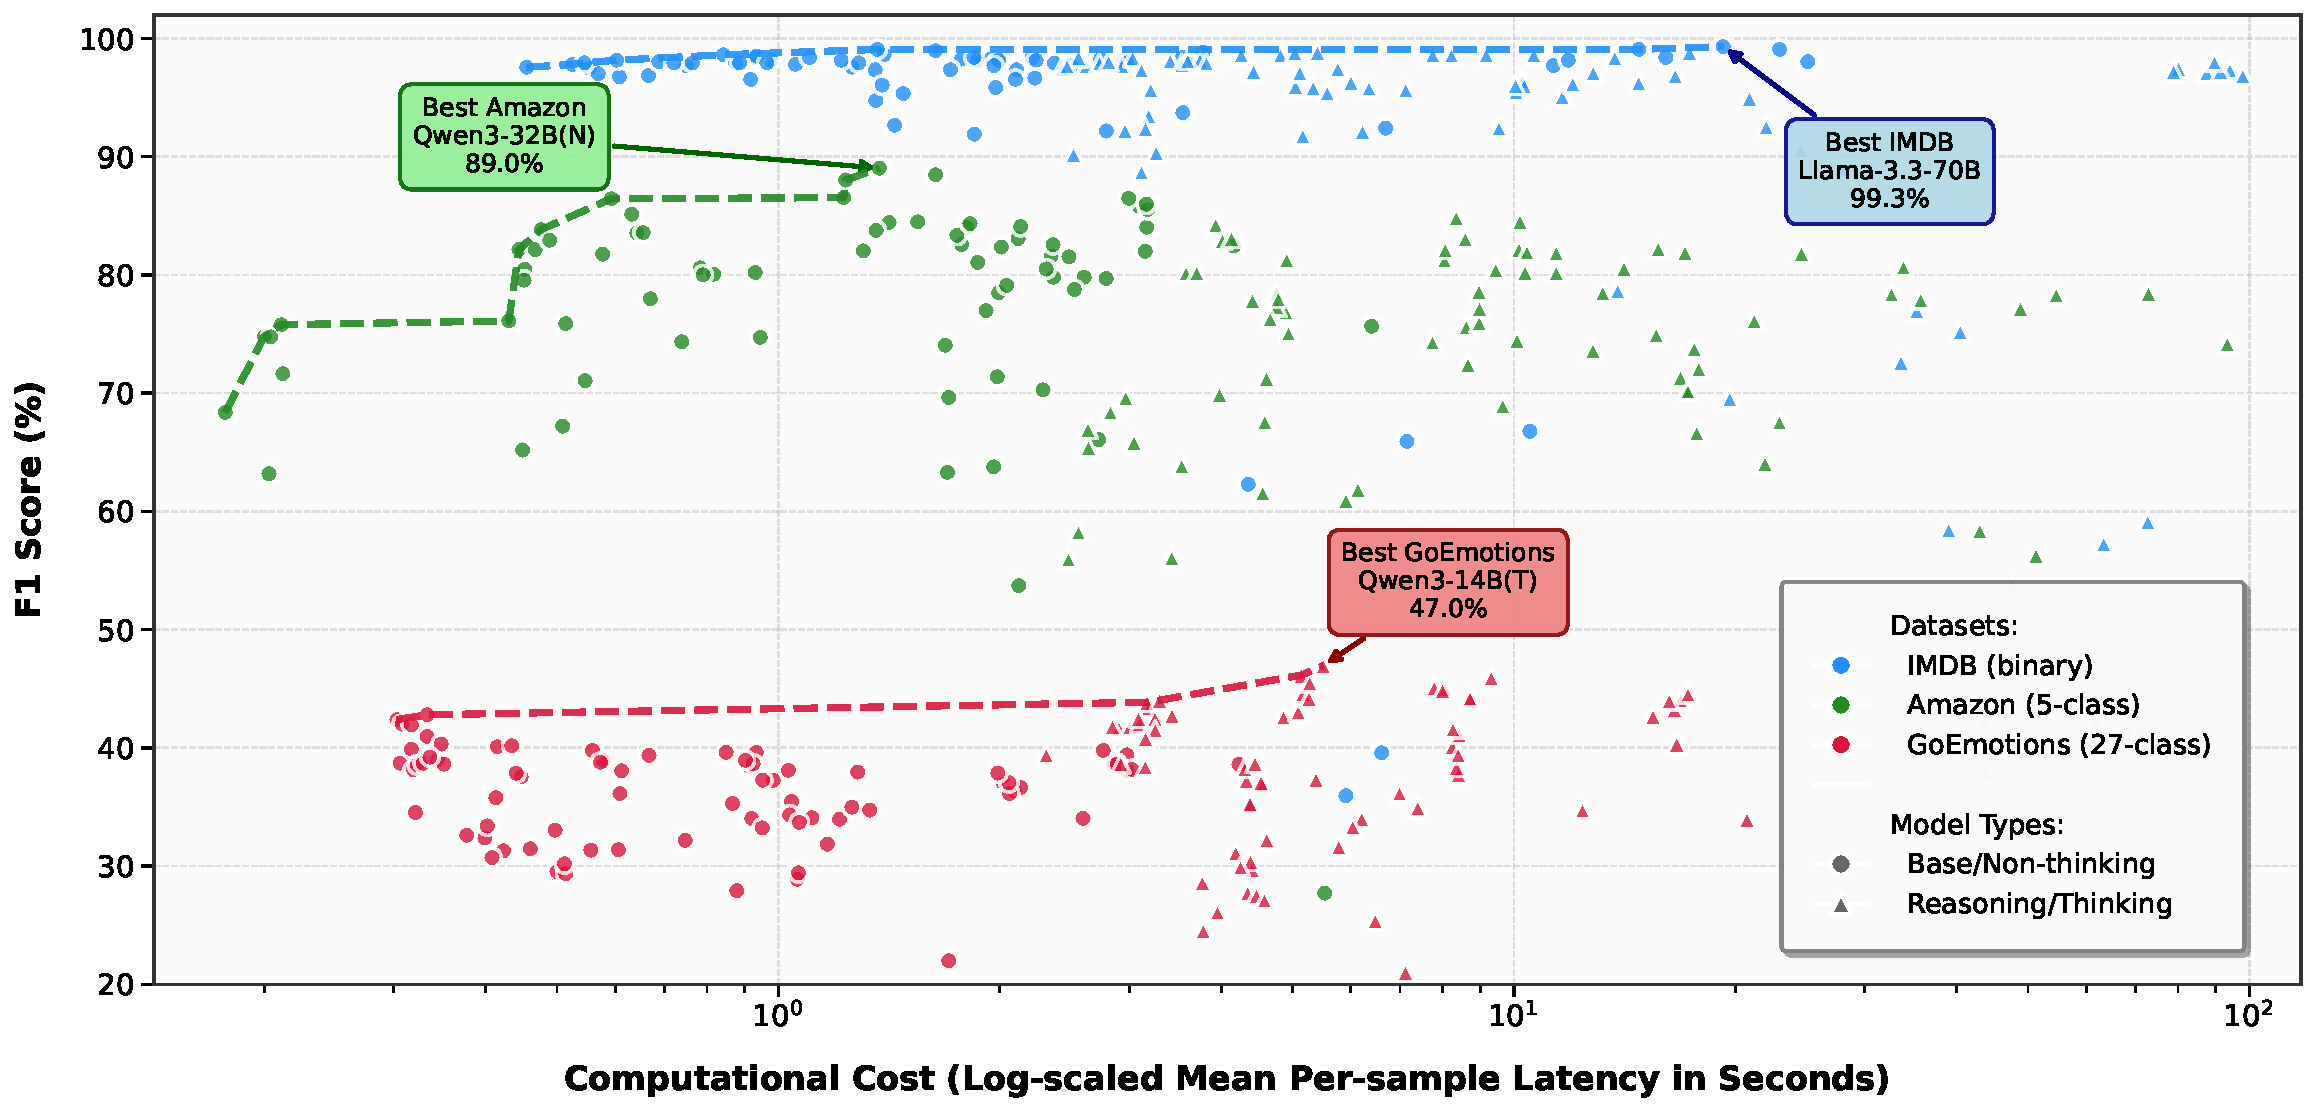
\includegraphics[width=\textwidth]{figures/pareto_frontier_v2.pdf}
\caption{Performance vs. computational cost. Circles: base/non-thinking; triangles: reasoning/thinking. Colors: IMDB (blue), Amazon (green), GoEmotions (red). Dashed lines: Pareto frontiers where no configuration dominates on both metrics. Evaluated on H100 via Ollama; DSR1/V3 excluded for consistency. Labels show top performers per dataset.}
\label{fig:pareto_frontier}
\end{figure}

Key observations from Pareto analysis:

\begin{enumerate}[leftmargin=*]
    \item \textbf{Task-dependent model representation:} IMDB frontier is dominated by base models achieving 97--99\% F1 with minimal latency. GoEmotions frontier includes reasoning models more frequently, justifying their overhead through accuracy gains.
    
    \item \textbf{Cost-performance curves:} IMDB shows flat frontier at high F1, indicating diminishing returns from additional compute. GoEmotions exhibits steeper slope, where latency increases yield greater accuracy improvements.
    
    \item \textbf{Practical guidance:} Base models dominate for most sentiment classification tasks. Reasoning should be reserved for complex emotion recognition where 2--4 pp improvements justify 2.1×--54× computational overhead.
\end{enumerate}

\subsubsection{Summary of Task Complexity Findings}

This comprehensive evaluation reveals that reasoning effectiveness in sentiment analysis is systematically task-dependent:

\begin{enumerate}[leftmargin=*]
    \item \textbf{Simple tasks (binary classification):} Base/non-thinking models provide superior performance (4.8 pp advantage) with lower computational overhead. Reasoning introduces noise rather than clarification.
    
    \item \textbf{Moderate tasks (5-class sentiment):} Mixed results with 3.6 pp average base model advantage. Reasoning can help disambiguate adjacent categories but may overcomplicate straightforward cases.
    
    \item \textbf{Complex tasks (27-class emotion):} Reasoning models achieve 2.0 pp advantage, with the lowest failure rate (14\%) among thinking vs. non-thinking comparisons. Extended reasoning helps navigate fine-grained distinctions between similar emotions.
    
    \item \textbf{Few-shot learning superiority:} Regardless of reasoning mode, few-shot learning yields improvements over zero-shot in the vast majority of cases, positioning it as a more robust strategy than reasoning activation for enhancing sentiment analysis performance.
\end{enumerate}

These findings provide principled deployment guidance: reserve reasoning for complex multi-class problems where accuracy gains justify computational overhead, and leverage few-shot learning for consistent improvements across all task complexities.

\section{Cross-Domain Applications}
\label{sec:cross_domain}

\subsection{Chinese-English Translation Optimization}
\label{subsec:translation}

\subsubsection{Motivation}

Machine translation between Chinese and English poses particular challenges due to significant differences in syntax, semantics, and morphology. Traditional approaches have struggled with complexities inherent in Chinese-English translation, particularly in handling idiomatic expressions, word order differences, and character-based text segmentation. We comprehensively evaluate LLMs across zero-shot, few-shot, and fine-tuned paradigms to establish best practices for practical deployment.

\subsubsection{Dataset}

We use the MAC (Manually Aligned Chinese-English) dataset\footnote{\url{https://github.com/bfsujason/mac}}, comprising parallel Mandarin-English texts from six Chinese novels representing diverse genres: humor, martial arts, classics, war, romance, and science fiction. After preprocessing to remove entries with missing content and splitting 80\%/20\%, the dataset contains 4,528 training and 1,133 testing sentence pairs.

\subsubsection{Evaluation Metrics}

\begin{enumerate}[leftmargin=*]
    \item \textbf{COMET-22:} Neural-based metric using contextual embeddings from pretrained language models. COMET-22 shows strong correlation with human judgments for Chinese-English translation, outperforming traditional metrics like BLEU and TER in alignment with human evaluations.
    
    \item \textbf{Translation Completeness Ratio (TCR):} During evaluation, we observed that some LLM outputs contained untranslated segments with Chinese characters. TCR measures the proportion of translations fully rendered into English:
    \begin{equation}
    TCR = \frac{\text{Number of complete translations}}{\text{Total number of entries}}
    \end{equation}
    where a ``complete translation'' is defined as one where no Chinese characters remain in the output text. This metric addresses a reliability dimension similar to VCR for classification tasks, capturing whether models produce deployable outputs.
    
    \item \textbf{Characters per Second (CPS):} Translation efficiency metric measuring processing speed:
    \begin{equation}
    CPS = \frac{\text{Number of Chinese characters in dataset}}{\text{Total translation time (seconds)}}
    \end{equation}
\end{enumerate}

\subsubsection{Results}

Table~\ref{tab:translation_results} presents translation performance across paradigms.

\begin{table}[htbp]
\centering
\caption{Chinese-English Translation Performance}
\label{tab:translation_results}
\begin{tabular}{@{}llcccc@{}}
\toprule
\textbf{Model} & \textbf{Paradigm} & \textbf{COMET} & \textbf{TCR (\%)} & \textbf{CPS} \\
\midrule
Qwen2-72B & Zero-shot & \textbf{0.7324} & 98.2 & 12.4 \\
GPT-4o & Zero-shot & 0.7258 & 99.1 & 18.2 \\
GPT-4o-mini & Zero-shot & 0.7259 & 98.8 & 24.5 \\
InternLM2.5-7B & Zero-shot & 0.7174 & 97.5 & 38.2 \\
Qwen2-7B & Zero-shot & 0.7170 & 97.8 & 35.6 \\
Llama-3.1-8B & Zero-shot & 0.7089 & 96.8 & 32.1 \\
Mistral-7B & Zero-shot & 0.6945 & 95.2 & 41.8 \\
Phi-3.5-mini & Zero-shot & 0.6823 & 94.5 & 45.2 \\
\midrule
Qwen2-72B & Fine-tuned & \textbf{0.7345} & 99.2 & 12.1 \\
Llama-3.1-70B & Fine-tuned & 0.7312 & 99.0 & 14.9 \\
InternLM2.5-7B & Fine-tuned & 0.7289 & 98.8 & 36.8 \\
Qwen2-7B & Fine-tuned & 0.7256 & 98.5 & 34.2 \\
Llama-3.1-8B & Fine-tuned & 0.7234 & 98.2 & 30.5 \\
Phi-3.5-mini & Fine-tuned & 0.7198 & 98.5 & 41.8 \\
Mistral-7B & Fine-tuned & 0.7145 & 97.8 & 39.5 \\
\bottomrule
\end{tabular}
\end{table}

Key findings:

\begin{enumerate}[leftmargin=*]
    \item \textbf{Zero-shot performance:} Qwen2-72B demonstrated the highest zero-shot performance (COMET 0.7324), followed closely by GPT-4o (0.7258) and GPT-4o-mini (0.7259). This suggests that models with strong multilingual pretraining can achieve competitive translation quality without task-specific examples.
    
    \item \textbf{Fine-tuning benefits:} Fine-tuning improves both translation quality and efficiency for open-source models. Fine-tuned Qwen2-72B achieves COMET 0.7345 with 99.2\% TCR, representing modest but consistent improvements. Notably, for all open-source LLMs, fine-tuning not only improves COMET scores but also increases CPS rates compared to few-shot learning.
    
    \item \textbf{Efficiency-quality trade-off:} Smaller fine-tuned models (Phi-3.5-mini, InternLM2.5-7B) offer 2--3$\times$ speed improvements with acceptable quality loss, suitable for high-throughput applications where perfect translation is not critical.
    
    \item \textbf{Optimal fine-tuning epochs:} Larger models peak earlier (2--3 epochs) than smaller ones (4--5 epochs), with training beyond optimal epochs leading to overfitting. This pattern is consistent with our findings in logical reasoning fine-tuning (Section~\ref{subsec:turtle_soup}).
    
    \item \textbf{LoRA/QLoRA effectiveness:} Parameter-efficient fine-tuning with LoRA/QLoRA enables the same LLM to be adapted for multiple tasks. Different adapters can be swapped for inference, creating a highly versatile solution without retraining entire models.
\end{enumerate}

\subsection{LLM Sentiment for Sports Betting Prediction}
\label{subsec:soccer_betting}

\subsubsection{Motivation}

Traditional sports betting models have primarily relied on quantitative statistics, often overlooking the predictive power of qualitative insights such as sentiment from match commentaries. We present a novel hybrid framework integrating LLM-derived sentiment features into machine learning models for soccer betting prediction, demonstrating that pre-trained LLMs can effectively capture latent factors often missed by traditional statistical methods.

\subsubsection{Methodology}

\textbf{Data Sources:}
\begin{itemize}[leftmargin=*]
    \item Match statistics from API-Football (2015-16 to 2023-24 seasons, 9 seasons)
    \item Betting odds from Football-Data.co.uk (1X2 pre-match odds from BetFair)
    \item Post-match commentaries from BBC Sport, scraped using Python Selenium
\end{itemize}

\textbf{Data Partitioning:} 2015--19 for feature selection/hyperparameter tuning; 2015--22 for training; 2022--23 for testing; 2023--24 for betting simulation.

\textbf{LLM Sentiment Analysis:} We employ zero-shot prompting with DeepSeek-R1, GPT-4o-mini, GPT-4.1, and Qwen2.5-Plus to extract sentiment ratings (1--5 scale: Strongly Negative to Strongly Positive) from match commentaries. The final sentiment feature is computed as the difference between home and away team ratings.

\textbf{Machine Learning Models:} Logistic Regression, SVC, Random Forest, and XGBoost, evaluated under both accuracy-tuned and F1-tuned configurations with grid search hyperparameter optimization and 5-fold cross-validation.

\textbf{Betting Strategy:} Simulated bankroll of \$10,000 using one-eighth Kelly betting criterion, placing bets only when positive expected value conditions are satisfied.

\subsubsection{Results}

Table~\ref{tab:soccer_results} presents betting simulation returns for the 2023-24 EPL season.

\begin{table}[htbp]
\centering
\caption{Soccer Betting Returns: Baseline vs. LLM-Enhanced Models (\%)}
\label{tab:soccer_results}
\begin{tabular}{@{}llcc@{}}
\toprule
\textbf{Model} & \textbf{LLM Enhancement} & \textbf{Accuracy-Tuned} & \textbf{F1-Tuned} \\
\midrule
Logistic Regression & Baseline & 75.12 & 105.22 \\
Logistic Regression & DeepSeek-R1 & 89.35 & \textbf{174.01} \\
Logistic Regression & GPT-4.1 & 79.52 & 60.02 \\
Logistic Regression & GPT-4o-mini & 27.10 & 110.64 \\
Logistic Regression & Qwen2.5-Plus & 41.98 & 75.04 \\
\midrule
SVC & Baseline & 72.18 & 33.07 \\
SVC & DeepSeek-R1 & 25.02 & 25.02 \\
SVC & GPT-4o-mini & 19.12 & 89.81 \\
\midrule
Random Forest & Baseline & -21.01 & 113.96 \\
Random Forest & GPT-4.1 & 7.32 & \textbf{279.48} \\
Random Forest & Qwen2.5-Plus & 65.54 & 74.04 \\
Random Forest & DeepSeek-R1 & 22.03 & 164.76 \\
\midrule
XGBoost & Baseline & 8.30 & \textbf{247.97} \\
XGBoost & DeepSeek-R1 & 92.07 & 33.15 \\
XGBoost & GPT-4o-mini & -5.55 & -16.09 \\
XGBoost & GPT-4.1 & 5.72 & 30.06 \\
\bottomrule
\end{tabular}
\end{table}

Key findings:

\begin{enumerate}[leftmargin=*]
    \item \textbf{F1 tuning superiority:} F1-tuned models consistently outperform accuracy-tuned configurations, with returns often 2--3$\times$ higher. This demonstrates that optimizing for balanced precision and recall is better aligned with profitable sports betting than accuracy optimization, as F1 tuning produces more calibrated probability estimates. This finding reinforces the broader dissertation theme that metric selection must align with downstream objectives.
    
    \item \textbf{Best performing configurations:}
    \begin{itemize}
        \item Random Forest + GPT-4.1 (F1-tuned): 279.48\% return---highest overall
        \item XGBoost Baseline (F1-tuned): 247.97\% return---strong baseline performance
        \item Logistic Regression + DeepSeek-R1 (F1-tuned): 174.01\% return---demonstrating that even simple models benefit from sentiment enhancement
        \item Random Forest + DeepSeek-R1 (F1-tuned): 164.76\% return
    \end{itemize}
    
    \item \textbf{LLM-model compatibility:} The impact of LLM-derived sentiment features varies across architectures. While certain combinations produce exceptional results (Random Forest + GPT-4.1), the same LLM can show different effects with different model architectures. Notably, XGBoost baseline outperforms some LLM-enhanced configurations, underscoring the importance of systematic empirical validation.
    
    \item \textbf{Zero-shot effectiveness:} Modern LLMs serve as powerful zero-shot sentiment analysis engines requiring no domain-specific training, enabling rapid deployment of sentiment-enhanced prediction systems. This demonstrates that thoughtful feature engineering with LLM-derived features can surpass architectural complexity.
\end{enumerate}

Figure~\ref{fig:betting_evolution} illustrates bankroll evolution across the 2023-24 season, demonstrating the superior stability and growth of F1-tuned models compared to accuracy-tuned alternatives.

\begin{figure*}[htbp]
\centering
\subfloat[Logistic Regression\label{fig:logistic_bankroll_f1}]{%
    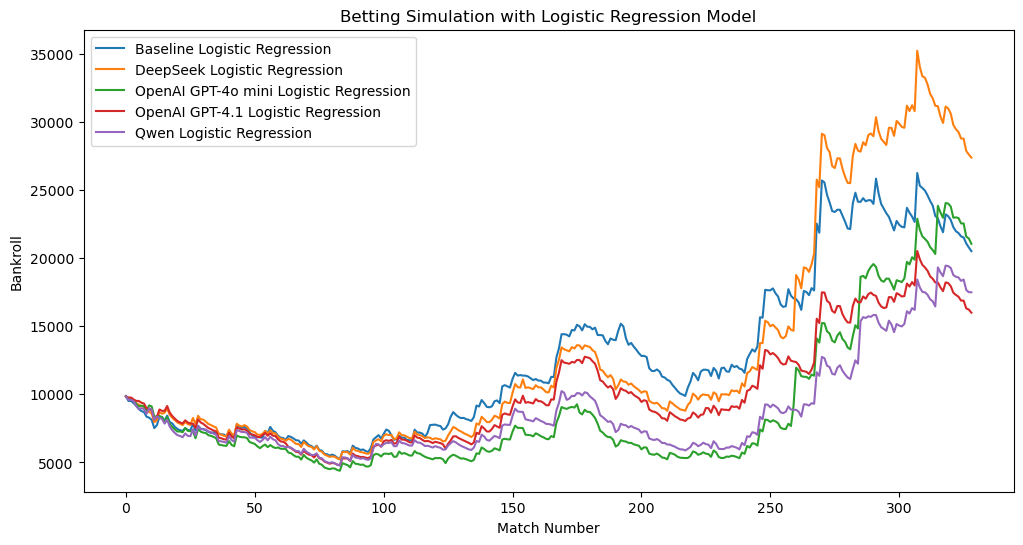
\includegraphics[width=0.48\textwidth]{images/lr_f1.png}
}
\hfill
\subfloat[SVC\label{fig:svc_bankroll_f1}]{%
    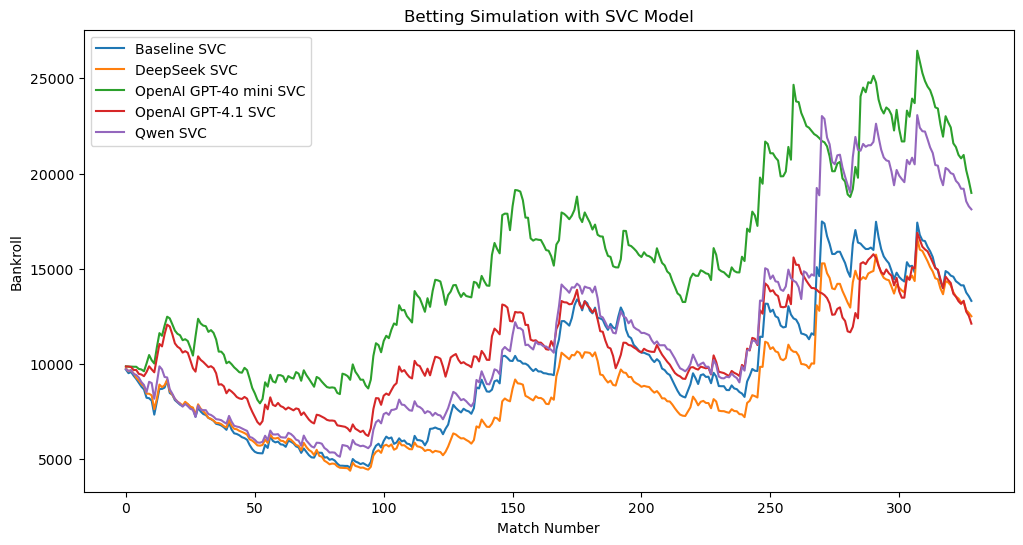
\includegraphics[width=0.48\textwidth]{images/svc_f1.png}
}

\vspace{0.1cm}

\subfloat[Random Forest\label{fig:random_forest_bankroll_f1}]{%
    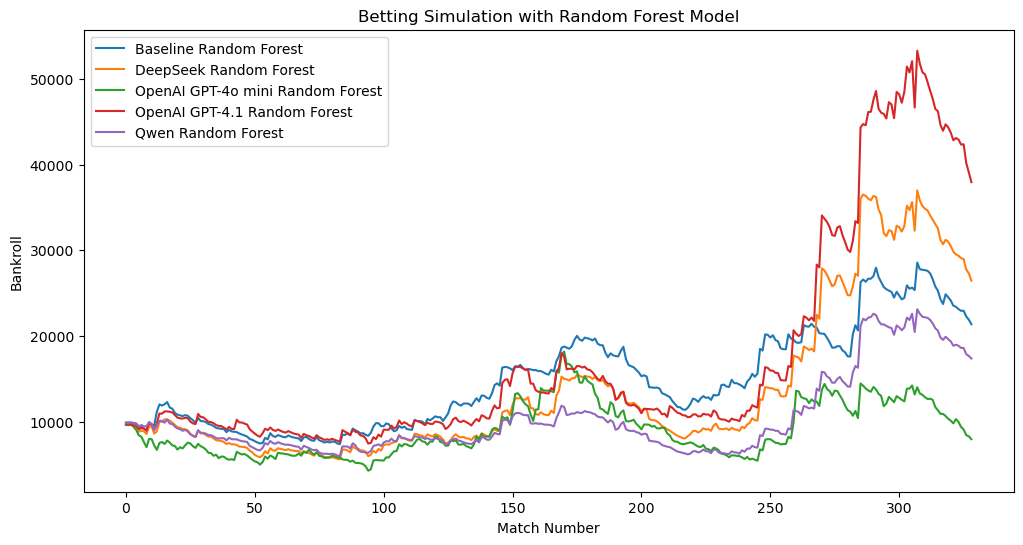
\includegraphics[width=0.48\textwidth]{images/rf_f1.png}
}
\hfill
\subfloat[XGBoost\label{fig:xgboost_bankroll_f1}]{%
    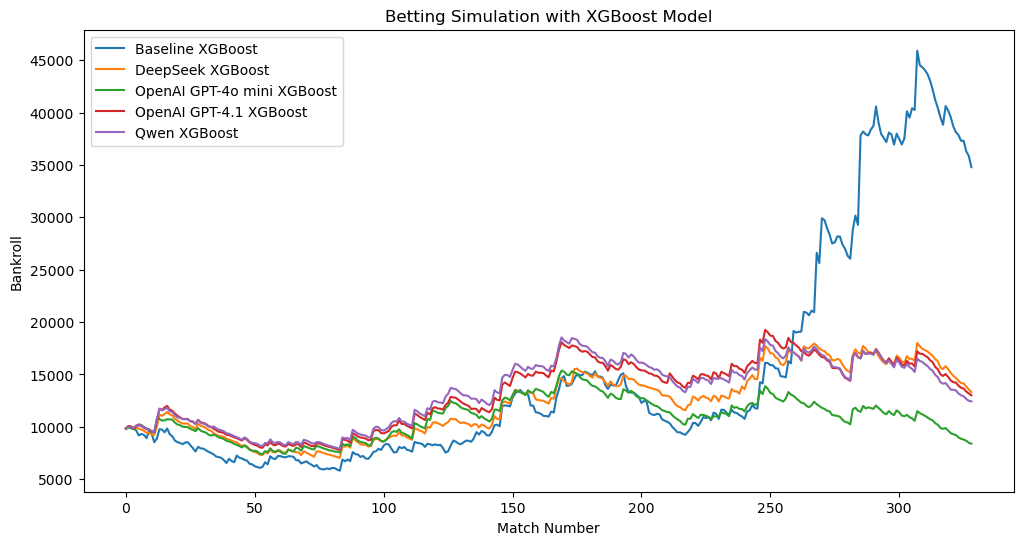
\includegraphics[width=0.48\textwidth]{images/xgboost_f1.png}
}

\caption{Betting simulation bankroll evolution across matches for the 2023-24 EPL season comparing F1-tuned baseline models with their LLM-infused variations across four different machine learning architectures. The results demonstrate that F1-tuned configurations consistently produce more stable growth trajectories and higher final returns.}
\label{fig:betting_evolution}
\end{figure*}

\section{Summary and Implications}
\label{sec:deployment_summary}

This chapter addressed RQ3 by examining deployment configurations, reasoning enhancement techniques, and application strategies that maximize LLM effectiveness across diverse enterprise use cases. The findings connect to and extend the optimization principles established in Chapters~\ref{ch:rag} and \ref{ch:agentic}, demonstrating their applicability across edge deployment, reasoning enhancement, and cross-domain applications.

\subsection{Edge Deployment Guidelines}

\begin{enumerate}[leftmargin=*]
    \item \textbf{Optimal model sizing:} Medium-sized models (7B--32B) achieve the best balance between performance and efficiency for edge deployment. qwen2.5:32b attains 96.75\% ($\pm$0.11\%) F1 with practical inference speeds, while smaller models like qwen2.5:3b achieve 90.89\% F1 with significantly lower resource requirements.
    
    \item \textbf{Quantization effectiveness:} Ollama's Q4\_K\_M quantization enables efficient deployment on consumer hardware while preserving or improving performance compared to bitsandbytes implementations (up to 3.37 percentage point F1 improvement observed).
    
    \item \textbf{Platform optimization:} WSL delivers up to 21$\times$ throughput improvements over native Windows for smaller models, enabling efficient deployment on consumer-grade systems without Linux installation.
    
    \item \textbf{Consumer hardware viability:} For reasoning tasks, models up to 14B parameters are feasible on 16GB consumer GPUs. qwen3:8b offers optimal accuracy-efficiency trade-offs (84.8\% F1, 13GB VRAM, 8.35s inference) for privacy-preserving local deployment.
    
    \item \textbf{Energy considerations:} Small models (1.5B--3B) achieve the highest performance-to-power ratios (0.161--0.163 \%/J), ideal for energy-constrained deployments, while large models (70B+) consume 1,283--1,876 Joules per inference.
\end{enumerate}

\subsection{Reasoning Enhancement Insights}

\begin{enumerate}[leftmargin=*]
    \item \textbf{Open-source competitiveness:} Fine-tuned Qwen2.5 and Llama3.1 models match or exceed GPT-4o on complex reasoning tasks. Qwen2.5-72B achieves 80.88\% F1 on TSQA with only 10-shot prompting, surpassing GPT-4o's 80.36\%. This extends the open-source viability findings from Chapter~\ref{ch:rag} to reasoning-intensive tasks.
    
    \item \textbf{Task-complexity-dependent reasoning effectiveness:} Comprehensive evaluation across 504 configurations reveals that reasoning effectiveness is systematically task-dependent. Base/non-thinking models outperform reasoning variants by $4.8 \pm 6.3$ pp on binary classification (IMDB) and $3.6 \pm 2.2$ pp on 5-class sentiment (Amazon), while reasoning models achieve $2.0 \pm 1.0$ pp advantage on 27-class emotion recognition (GoEmotions). This task-complexity hypothesis provides principled guidance: reserve reasoning for complex multi-class problems where accuracy gains justify 2.1×--54× computational overhead.
    
    \item \textbf{Distillation transfer limitations:} Reasoning patterns optimized for mathematical and logical tasks transfer poorly to simpler sentiment classification. Failure rates decrease with task complexity: 100\% (IMDB), 80\% (Amazon), 50\% (GoEmotions), indicating reasoning distillation becomes more beneficial as classification granularity increases.
    
    \item \textbf{Valid Classification Ratio (VCR):} Novel metric for assessing output reliability beyond accuracy, particularly important for structured classification tasks where invalid outputs cause downstream failures. Fine-tuning improves VCR to $>$98.6\% across evaluated models, with some models improving from as low as 1.17\% to 100\% within 0.2 epochs.
    
    \item \textbf{Reasoning Intensity (RI):} Novel metric capturing the trade-off between explanation depth and computational cost. Three operational regimes identified: Minimal (RI $<$ 0.5), Balanced (0.5--0.85), and Intensive ($>$ 0.85), with balanced regime yielding optimal accuracy-efficiency trade-offs.
    
    \item \textbf{Explainability benefits:} DeepSeek-R1's intrinsic reasoning traces provide transparent decision-making processes without external explanation mechanisms, enhancing auditability for enterprise applications.
    
    \item \textbf{Few-shot learning superiority:} Few-shot learning yields improvements over zero-shot in the vast majority of cases, regardless of reasoning mode, positioning it as a more robust and consistent strategy than reasoning activation for enhancing sentiment analysis performance. DeepSeek-R1 demonstrates approximately 8$\times$ improvement in few-shot efficiency over GPT-4o (30 shots vs. 40 shots for comparable performance).
    
    \item \textbf{Pareto-optimal model selection:} Pareto frontier analysis reveals that base models dominate efficiency-performance trade-offs for most sentiment tasks. IMDB frontier is dominated by base models achieving 97--99\% F1 with minimal latency, while GoEmotions includes reasoning models that justify overhead through accuracy gains.
    
    \item \textbf{Temporal robustness challenges:} All evaluated models exhibit 10--17 percentage point F1 degradation on contemporary data, though reasoning intensity remains stable ($\pm$0.02). This suggests models require periodic updating to maintain accuracy on evolving content.
\end{enumerate}

\subsection{Cross-Domain Application Patterns}

\begin{enumerate}[leftmargin=*]
    \item \textbf{Fine-tuning universality:} Parameter-efficient fine-tuning (LoRA/QLoRA) consistently improves performance across translation, reasoning, and sentiment tasks. The technique enables multi-task adaptation through swappable adapters without full model retraining.
    
    \item \textbf{Zero-shot LLM capabilities:} Modern LLMs effectively extract nuanced signals from unstructured text without domain-specific training, enabling rapid deployment across diverse domains. This was demonstrated in both Chinese-English translation (COMET 0.7324 for Qwen2-72B) and sports sentiment extraction.
    
    \item \textbf{Optimization strategy alignment:} Task-specific optimization dramatically improves practical outcomes. F1 tuning for sports betting produces 2--3$\times$ higher returns than accuracy tuning, demonstrating that metric selection must align with downstream objectives.
    
    \item \textbf{Novel evaluation metrics:} This chapter introduces four domain-specific metrics, complementing the RAP metric from Chapter~\ref{ch:rag} and the ASR/ECR@1 metrics from Chapter~\ref{ch:agentic}:
    \begin{itemize}
        \item \textbf{VCR} (Valid Classification Ratio) for output reliability in classification tasks
        \item \textbf{RI} (Reasoning Intensity) for reasoning-explainability trade-offs
        \item \textbf{TCR} (Translation Completeness Ratio) for translation reliability
        \item \textbf{CPS} (Characters per Second) for translation efficiency
    \end{itemize}
\end{enumerate}

These findings provide practitioners with evidence-based guidelines for deploying LLMs across diverse enterprise contexts, balancing performance, efficiency, explainability, and cost considerations. The research demonstrates that open-source models can achieve enterprise-grade performance when properly optimized, enabling privacy-preserving edge deployment while maintaining competitive accuracy with proprietary alternatives.